\section{近似解与计算评价}
\label{sec:opt-prob-approximation}

前四节讨论的是精确的最优解。实际计算几乎从不交出精确解：迭代在有限步后停止，浮点运算带来舍入，数据本身也有误差。于是需要回答一个新问题：在给定预算内得到的结果，好到什么程度？这个问题有两个维度。结果误差规定“有多准”，计算成本规定“为此付出多少”。本节为后续各章建立共同的评价语言；具体的误差界、停止规则和误差传播，随相应方法在各章展开。

\subsection{目标误差、解误差与最优性残差}
\label{sec:opt-prob-error-measures}

\paragraph{三种误差}
设$\hat{\bm x}\in C$是交出的可行近似解，最优值$f^\star$有限，最优解集合$S=\argmin_{\bm x\in C}f$非空。至少有三种量可以衡量它的好坏。

\begin{itemize}
  \item 目标差$f(\hat{\bm x})-f^\star\geq0$：结果比最优值差多少。若$f(\hat{\bm x})-f^\star\leq\varepsilon$，称$\hat{\bm x}$为目标值意义下的$\varepsilon$近似解。
  \item 到解集的距离$\operatorname{dist}(\hat{\bm x},S)=\inf_{\bm x\in S}\lVert\hat{\bm x}-\bm x\rVert_2$：参数离最优解有多远。最优解唯一时就是$\lVert\hat{\bm x}-\bm x^\star\rVert_2$。
  \item \term{最优性残差}（optimality residual）：在$\hat{\bm x}$处可以直接计算、并在最优解处为零的量。对无约束可微问题，最常用的是梯度范数$\lVert\nabla f(\hat{\bm x})\rVert_2$。
\end{itemize}

前两种量都含有未知的$f^\star$或$S$，求解过程中通常算不出来；第三种量能算，但它与前两者的关系需要额外条件。三者不能互相代替。

\paragraph{平坦目标中小梯度不等于小误差}
图~\ref{fig:opt-prob-flat-gradient}(a)比较两个一元二次函数$f_1(x)=0.01x^2/2$与$f_2(x)=x^2/2$，最小点都是$0$，最优值都是$0$。在$x=10$处$f_1'(10)=0.1$，在$x=0.1$处$f_2'(0.1)=0.1$，两个点的梯度一样小。但前者的目标差是$0.5$、到最小点的距离是$10$，后者分别是$0.005$和$0.1$，相差两个数量级。原因在于曲率：$f_1$的二阶导数只有$0.01$，地形太平，坡度很小时离谷底仍然很远。

\begin{figure*}[!htbp]
  \centering
  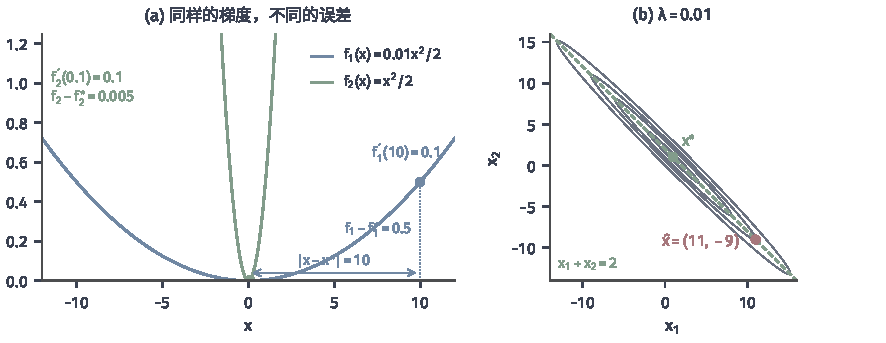
\includegraphics[width=150mm]{figures/03-optimization-evolution-and-signals/01-optimization/matplotlib/c1-flat-gradient/figure.pdf}
  \caption{小梯度与小误差。(a) 平坦的$f_1(x)=0.01x^2/2$（蓝）在$x=10$处与陡峭的$f_2(x)=x^2/2$（绿）在$x=0.1$处有相同的导数$0.1$，但$f_1$的目标差为$0.5$、到最小点的距离为$10$，$f_2$分别只有$0.005$和$0.1$。(b) 最小二乘实例取$\lambda=0.01$，灰线是$f-f^\star=0.1,0.5,1,2$的等值线，沿绿色虚线$x_1+x_2=2$极度拉长。$\hat{\bm x}=(11,-9)$（红点）的观测残差为零、梯度范数约$0.142$，但目标差约为$1.00$，到$\bm x^\star\approx(0.995,0.995)$的距离约为$14.1$。}
  \label{fig:opt-prob-flat-gradient}
\end{figure*}

\paragraph{小观测误差不等于小参数误差}
最小二乘实例给出多维的版本。先取$\lambda=0$。点$\hat{\bm x}=(11,-9)$满足$11+(-9)=2$，观测残差$\bm A\hat{\bm x}-\bm b=0$，它本身就是一个最优解，到最优解集合的距离为$0$。但如果我们心里的“正确参数”是$(1,1)$，两者相距$\lVert(10,-10)\rVert_2\approx14.1$。可见在解不唯一时，“参数误差”必须说明参照的是解集合还是某个指定的解；观测拟合得再好，也不能告诉我们数据没有约束的方向。

再取$\lambda=0.01$，问题有唯一解$\bm x^\star=\frac{2}{2.01}(1,1)\approx(0.995,0.995)$，最优值$f^\star=\frac{0.01\cdot4}{2\cdot2.01}\approx0.00995$。对同一个$\hat{\bm x}=(11,-9)$，观测残差仍为零，梯度$\nabla f(\hat{\bm x})=\bm A^\top(\bm A\hat{\bm x}-\bm b)+\lambda\hat{\bm x}=(0.11,-0.09)$，范数约为$0.142$；目标值$f(\hat{\bm x})=0.005\cdot(121+81)=1.01$，目标差约为$1.00$；到$\bm x^\star$的距离约为$14.1$。图~\ref{fig:opt-prob-flat-gradient}(b)显示了原因：强凸常数$\mu=\lambda=0.01$很小，等值线沿$(1,-1)$方向被拉得极长，$\hat{\bm x}$虽在谷底的“长沟”里，却离真正的最低点很远。

\paragraph{残差何时能控制误差}
强凸性给出了从残差到误差的换算。设$f$在$\mathbb R^d$上可微且$\mu$强凸。在式~\eqref{eq:opt-prob-strong-first-order}中取$\bm u=\hat{\bm x}$，右端是$\bm v$的二次函数，它在$\bm v=\hat{\bm x}-\nabla f(\hat{\bm x})/\mu$处取得最小值$f(\hat{\bm x})-\lVert\nabla f(\hat{\bm x})\rVert_2^2/(2\mu)$，所以对所有$\bm v$，$f(\bm v)$都不低于这个数，特别地对$\bm v=\bm x^\star$：
\[
  f(\hat{\bm x})-f^\star\leq\frac{\lVert\nabla f(\hat{\bm x})\rVert_2^2}{2\mu}.
\]
再结合定理~\ref{thm:opt-prob-strong-growth}，又得$\lVert\hat{\bm x}-\bm x^\star\rVert_2\leq\lVert\nabla f(\hat{\bm x})\rVert_2/\mu$。代入上面的数值：$0.142^2/(2\cdot0.01)\approx1.01$，确实不小于实际目标差$1.00$；$0.142/0.01\approx14.2$，确实不小于实际距离$14.1$。两个界都成立且接近实际值，但它们都被$1/\mu$放大：$\mu$越小，同样大小的梯度允许越大的误差。没有$\mu$这样的常数，小梯度不能推出任何关于目标差或距离的结论；这正是图~\ref{fig:opt-prob-flat-gradient}要说明的。

\paragraph{实验评价与停止判据}
要区分两种使用场合。在实验评价中，我们常对同一问题先用高精度方法（例如直接解正规方程）算出参照最优值$f^\star$或参照解，再画出目标差或距离随计算量的变化；这适合比较方法，但参照值本身也有误差，应当说明它是怎样得到的。在实际求解中，$f^\star$未知，只能依据可计算的残差决定何时停止，例如“梯度范数低于$\varepsilon$”；它对目标差的含义取决于是否有$\mu$这类条件。约束问题还要同时检查约束违背程度，非光滑问题要用替代梯度的量，而对偶间隙能直接给出目标差的上界；这些残差分别在第~\ref{chap:opt-nonsmooth}章与第~\ref{chap:constrained-optimization}章建立后才能使用，本章不提前使用它们。

\subsection{迭代次数与总计算成本}
\label{sec:opt-prob-cost}

\paragraph{先固定比较的对象}
后续章节的方法都产生一列迭代$\bm x^{(t)}$，$t=0,1,2,\dots$，并用某个误差$e^{(t)}\geq0$描述第$t$轮的质量。$e^{(t)}$可以是目标差、到解集的距离，也可以是某种残差；比较两个方法前，必须先说清比较的是哪一个。上面的例子已经表明，三者可以相差几个数量级。

\paragraph{三类收敛结论}
关于$e^{(t)}$的结论有强弱之分。
\begin{itemize}
  \item 渐近收敛：$e^{(t)}\to0$。它只说最终会任意准，不说要多少轮。
  \item 有限步误差界：对所有$t$都有可计算的上界$e^{(t)}\leq B(t)$。若$B(t)=c/(t+1)$之类按幂次下降，称为\term{次线性收敛}（sublinear convergence）；若$B(t)=c\rho^t$，$0<\rho<1$，称为\term{线性收敛}（linear convergence），在对数坐标中是一条直线。
  \item 局部收敛阶：若$e^{(t)}\to0$，且存在$M>0$、$p>1$，使$t$充分大后$e^{(t+1)}\leq M(e^{(t)})^p$，称收敛阶为$p$；$p=2$时称为\term{二次收敛}（quadratic convergence）。这类结论通常只在解的附近成立，不说明从远处出发要走多久。
\end{itemize}

由这些结论可以反推达到精度$\varepsilon$所需的轮数。线性收敛$c\rho^t\leq\varepsilon$需要$t\geq\log(c/\varepsilon)/\log(1/\rho)$，与$\log(1/\varepsilon)$成正比；次线性的$c/(t+1)\leq\varepsilon$需要约$c/\varepsilon$轮；二次收敛从$e^{(0)}=0.5$、$M=1$出发有$e^{(t)}=0.5^{2^t}$，只需约$\log_2\log_2(1/\varepsilon)$轮。图~\ref{fig:opt-prob-convergence-cost}(a)画出了三条由公式生成的误差序列：$1/(t+1)$、$0.9^t$与$e^{(t+1)}=(e^{(t)})^2$。要达到$\varepsilon=10^{-8}$，它们分别需要约$10^8$轮、$175$轮与$5$轮。收敛速率的这些定义沿用数值优化的通行用法\scite{math-nocedal2006numerical}。

\paragraph{每轮代价}
轮数只是一半。每一轮要做什么、花多少，取决于方法使用的计算单元。常见的单元有：求一次函数值，求一次梯度，做一次矩阵向量乘积，或者精确求解一个子问题。以稠密的$\bm A\in\mathbb R^{n\times d}$为例，最小二乘的一次函数值需要算$\bm A\bm x$，约$nd$次乘加；一次梯度$\bm A^\top(\bm A\bm x-\bm b)+\lambda\bm x$需要两次矩阵向量乘积，约$2nd$次乘加；若要直接解正规方程，形成$\bm A^\top\bm A$约需$nd^2$次乘加的量级，再对$d\times d$矩阵作Cholesky分解约需$d^3/3$次运算的量级。存储量也要登记：存$\bm A$需要$nd$个数，存$\bm A^\top\bm A$需要$d^2$个数。

\paragraph{总成本}
把两部分合起来，
\[
  \text{总成本}\approx\text{准备代价}+\text{每轮代价}\times\text{达到精度}\ \varepsilon\ \text{所需的轮数}.
\]
图~\ref{fig:opt-prob-convergence-cost}(b)把(a)中的线性序列和二次序列改按累计代价画出，假设前者每轮代价为$1$、后者为$40$。按轮数看，二次序列遥遥领先；按总代价看，达到$10^{-8}$时线性序列花$175$、二次序列花$5\times40=200$，前者反而更省；要求提高到$10^{-12}$时，二次序列只需$6$轮共$240$，线性序列需要$263$，二者又调换了位置。哪一个更划算，同时取决于精度要求和每轮代价。

\begin{figure*}[!htbp]
  \centering
  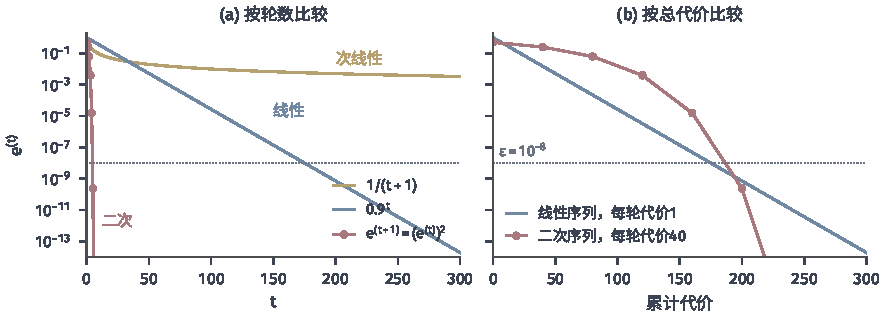
\includegraphics[width=150mm]{figures/03-optimization-evolution-and-signals/01-optimization/matplotlib/c1-convergence-cost/figure.pdf}
  \caption{收敛速率与总代价。三条曲线是由公式生成的误差序列，不是某个算法的实测结果，纵轴为对数刻度，灰色点线标出$\varepsilon=10^{-8}$。(a) 按轮数：次线性$1/(t+1)$（黄）、线性$0.9^t$（蓝）、二次$e^{(t+1)}=(e^{(t)})^2$且$e^{(0)}=0.5$（红）。(b) 按累计代价：线性序列每轮代价$1$，二次序列每轮代价$40$；达到$10^{-8}$分别需要$175$与$200$，达到$10^{-12}$分别需要$263$与$240$。}
  \label{fig:opt-prob-convergence-cost}
\end{figure*}

这给后续各章立下一条比较规则：比较两个方法时，应采用相同的问题、相同的误差对象、相同的精度要求和相同的输入规模，把每轮代价与轮数一起报告，必要时登记存储量。“二阶方法”“加速方法”这样的名称描述的是更新的构造方式，不能直接断定总效率更高；第~\ref{chap:opt-smooth}章起，每个方法都按这一口径给出输入、每轮代价与误差界。
